\begin{center}
\footnotesize\noindent\fbox{
	\parbox{\textwidth}{
	 Utilizzando Matlab, si costruisca una tabella dove, per \(h=10^{-j}, j=1,\ldots,10\) e per la funzione \(f(x)=x^4\) si riporta il valore di \(\phi_h(x)\) definito nell'Esercizio 2 in \(x=1\). Commentare i risultati ottenuti.
	}
}\end{center}

Il seguente codice Matlab soddisfa la richiesta. Di seguito si mostra la rappresentazione grafica della tabella ottenuta.
\\

\lstinputlisting[language=Matlab]{cap1/es3.m}

\begin{center}
	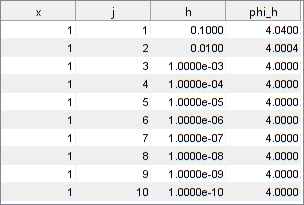
\includegraphics[scale=1]{cap1/es3.png}
\end{center}

\noindent Questi risultati verificano che, per valori sufficientemente piccoli di \(h\), il rapporto incrementale \(\phi_h(x) \approx f'(x)\) in quanto \(f'(x) = 4x^3\).
